\section{Пример построения временной диаграммы}
\sectionmark{Пример построения временной диаграммы}

\subsection{Построения временной диаграммы с помощью стилевого пакета ''tikz-timing''}


\begin{figure}[H]\center
  \captionsetup{singlelinecheck=true} %центрируем подрисуночную подпись

\newcommand{\timemeasure}[4]
{       \draw [red,semithick] ($ (#1) - (-0.1,0) $) -- ($ (#1) - (-0.1,#3) -(0,1) $);
        \draw [red,semithick] ($ (#2) - (-0.1,0) $) -- ($ (#2) - (-0.1,#3) -(0,1) $);
	\draw [red,semithick,<->] ($ (#1) - (-0.1,#3) $) -- ($ (#2) - (-0.1,#3) $) node [below,midway] {#4};
}

\newcommand{\timemeasureI}[2]
{       \draw [orange,semithick]  (#1) ellipse (.2 and .8) (#2) ellipse (.2 and .8) ;

}

 
%Define different DRAM commands:
\tikztimingmetachar{A}{1.0D{\texttt{ACT}}}
\tikztimingmetachar{O}{1.0D{\texttt{NOP}}}
\tikztimingmetachar{R}{1.0D{\texttt{RD}}}
\tikztimingmetachar{W}{1.0D{\texttt{WR}}}
 
\begin{tikztimingtable} [timing/d/background/.style={fill=white}, timing/lslope=0.2, xscale=2, yscale=1,]
        CLK & L N(P1) 6{T} N(P2) 2{T} L \\
        CMD & 0.5U A 1U O 1U O 1U R 2.5U\\
        ADD & 0.5U 1D{\footnotesize \texttt{B0}} 5U 1D{\footnotesize \texttt{B0}} 2.5U\\
        $~$ & \\
        TLM & 2z 6D{ ACT } 6z\\
        $~$ & 14z N(P3)3D{ RD }\\
   \extracode
   \begin{pgfonlayer}{background}
 
 
     \timemeasure{P1}{P2}{5}{\tiny $t_{RCD}$}
 
     \timemeasureI{P2}{P3}

 
     % Add vertical lines 
     \begin{scope}[semitransparent,semithick]
       \vertlines[gray]{1.1,3.1,...,9.1}
     \end{scope}
  \end{pgfonlayer}
\end{tikztimingtable}%

\caption{Временная диаграмма сигналов на системной шине} \label{p:time_tikz}
\end{figure}



%\begin{figure}[!h]\center
%  \captionsetup{singlelinecheck=true} %центрируем подрисуночную подпись
%\begin{tikzpicture}[timing/picture,thick, timing/nodes/advanced]
%  \timing at(0 ,2)                    {hH N(A) LHLHL};
%  \timing [timing/slope=.25] at(0,0)  {HLL N(B) HHLl};
%  \draw [orange, semithick] (A.mid) ellipse (.2 and .6) (B.mid) ellipse (.2 and .6);
%  \draw [orange, semithick ,->] ($ (A. mid ) - (0 ,.6) $) parabola [ bend pos =0.5] ($ (B. mid ) + (0 ,.6) $);
%\end{tikzpicture}
%\caption{Событийная зависимость между сигналами} \label{p:time_tikz_1}
%\end{figure}





\subsection{Включение временной диаграммы, сделанной в ''TimingAnalyzer''}


\begin{figure}[H]\center
  %  \captionsetup{singlelinecheck=true} %центрируем подрисуночную подпись
  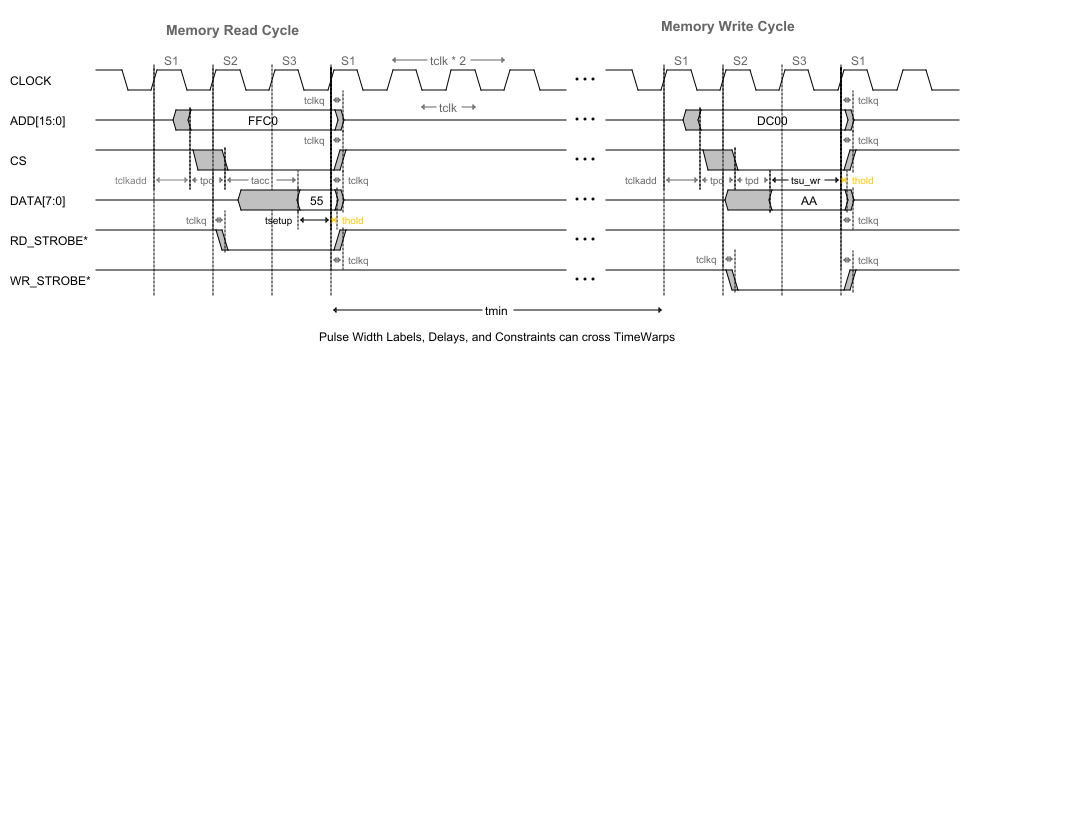
\includegraphics[width=1\textwidth]{./about/TimingAnalyzer/cnstrnt_err_int} % width=\textwidth
  %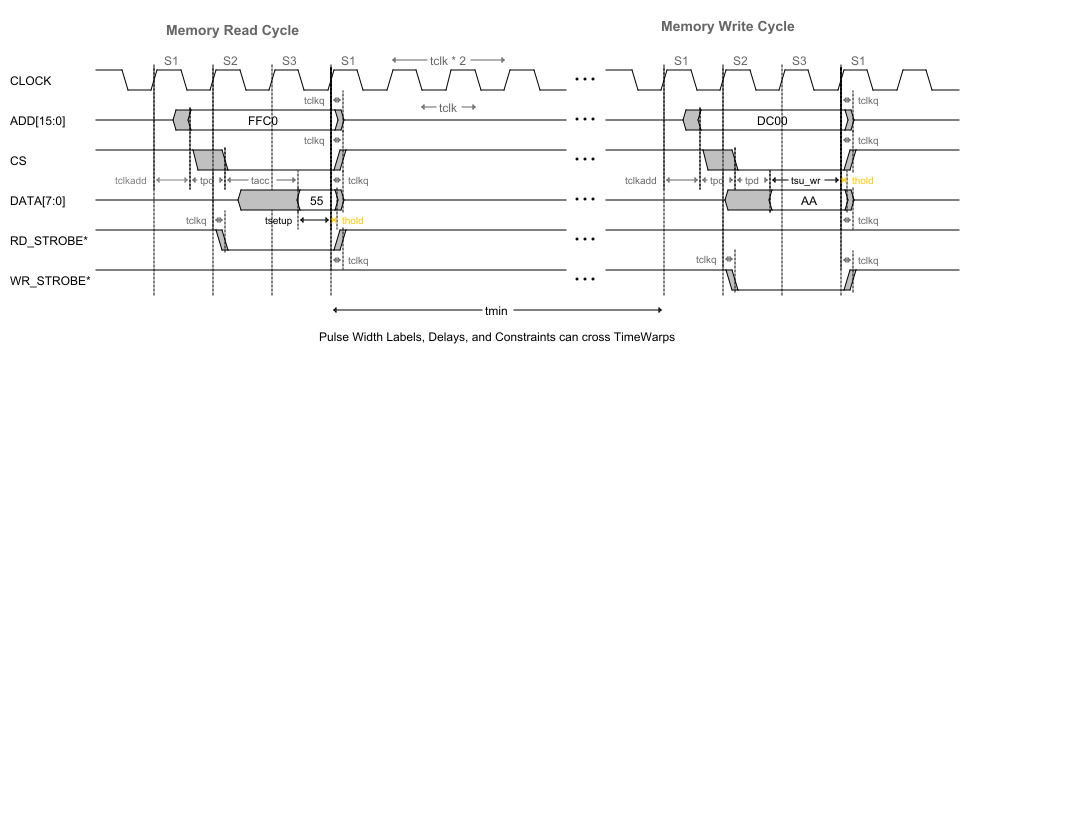
\includegraphics[trim=-5 -5 16 16,clip scale=0.5, width=150mm, height=50mm, keepaspectratio]{./about/TimingAnalyzer/cnstrnt_err_int}
  \caption{Временная диаграмма, сделанная в ''TimingAnalyzer v0.981'' и распечатанная в *.jpg (в *.pdf - формате вместо рисунка был белый фон). Мелкие символы размазаны} \label{p:time_TimingAnalyzer_1}
\end{figure}






\begin{figure}[H] \centering
\input ./about/TimingAnalyzer/cnstrnt_err_int_to_inkskape.tex
\caption{Временная диаграмма, сделанная в ''TimingAnalyzer v0.981'' -> *.svg -> ''Inkscape'' -> подогнан размер страницы к содержанию -> *.tex. Мелкие символы не размазаны}
\label{p:time_TimingAnalyzer_inkscape}
\end{figure}




%\begin{figure}[H] \centering
%\immediate\write18{inkscape -g -D --file=d:/yra/LaTeX/eskdi/about/TimingAnalyzer/cnstrnt_err_int.svg     --export-pdf=d:/yra/LaTeX/eskdi/about/TimingAnalyzer/cnstrnt_err_int_tex1.pdf}
%\immediate\write18{%
%psv.exe}
%echo "hello" > file1.tex}
%\includegraphics[width=1\textwidth]{./about/TimingAnalyzer/cnstrnt_err_int_tex1.pdf}
%\caption{Временная диаграмма, сделанная в ''TimingAnalyzer v0.981'' -> *.svg -> ''Inkscape'' -> подогнан размер страницы к содержанию -> *.tex. Мелкие символы не размазаны}
%\label{p:time_TimingAnalyzer_inkscape}
%\end{figure}




%\begin{figure}[H] \centering
%\includesvg[width=1\textwidth]{./about/TimingAnalyzer/cnstrnt_err_int11}
%\caption{Временная диаграмма, сделанная в ''TimingAnalyzer v0.981'' -> *.svg -> ''Inkscape'' -> подогнан размер страницы к содержанию -> *.tex. Мелкие символы не размазаны}
%\end{figure}















